\documentclass{beamer}
\usetheme{Berkeley}
\usecolortheme{dolphin}

\usepackage{tipa}
\usepackage{qtree}
\usepackage{ccicons}
\usepackage{hyperref}

\title{\LaTeX\ for Linguists}
\institute{Graduate Linguistics Student Association\\Research Tool Workshop Series\\Georgetown University\\jeh241@georgetown.edu}
\author{Jonathan Havenhill}
\date{\today}

\begin{document}

\frame{\titlepage
\begin{flushright}\ccbyncsa\end{flushright}}

\frame{\scriptsize\tableofcontents}

\section*{Files for today}
\begin{frame}[fragile]
\frametitle{Files for today}
\begin{itemize}
	\item <1-> You should download the following files:
	\item <1-> \url{github.com/jhavenhill/latex-for-linguists}
	\item <2-> If you don't have \LaTeX\ installed, you should download it:
	\begin{itemize}
		\item <2-> MikTeX for Windows
		\item <2-> MacTeX for Mac
		\item <2-> Or, sign up for a free account at \url{writelatex.com}
	\end{itemize}
\end{itemize}

\end{frame}

\section{Introduction}
\subsection{What is \LaTeX ?}

\begin{frame}[fragile]
\frametitle{Some basic information}

\begin{itemize}
\item <1-> First, how do you pronounce \LaTeX ?

\begin{itemize}
\item Usually \textipa{[leItEk]} or \textipa{[lA:tEk]}
\end{itemize}

\item <2-> It's a typesetting system, not a word processor

\item <3-> \LaTeX\ documents are written with markup code, which is then interpreted and compiled by the \TeX\ system

\item <4-> It has a learning curve, but there are a number of advantages, which you will hopefully see\ldots

\end{itemize}
\end{frame}

\subsection{The basics}

%Structure
\begin{frame}[fragile]
\frametitle{The structure of a \LaTeX\ document}

\begin{itemize}

\item <1-> Every document must contain the following lines:

\begin{verbatim}
\documentclass{...}
...
\begin{document}
...
\end{document}
\end{verbatim}
\end{itemize}

\end{frame}

%Hello World
\begin{frame}[fragile]
\frametitle{Let's start with a basic document}

\begin{verbatim}
\documentclass{article}

\begin{document}
Hello world!
\end{document}
\end{verbatim}

\end{frame}

%Document Class
\begin{frame}[fragile]
\frametitle{\textbackslash documentclass\{\}}

\begin{itemize}
\item <1-> The document classes you are most likely to use are:

\begin{itemize}
\item \texttt{article} (for articles)
\item \texttt{beamer} (for slideshows like this) 
\item \texttt{res} (for r\'esum\'es and CVs)
\end{itemize}

\item <2-> The \texttt{\textbackslash documentclass} command can have options, which are specified as such:

\begin{verbatim}
\documentclass[10pt,a4paper,landscape]{article}
\end{verbatim}

\end{itemize}

\end{frame}

%Preamble
\begin{frame}[fragile]
\frametitle{The preamble}

\begin{itemize}
\item <1-> The preamble comes between `documentclass\{\}' and `begin\{document\}'
\item <2-> Here, you list the packages you will be using, e.g.:

\begin{verbatim}
\documentclass{article}

\usepackage{covington}
\usepackage{qtree}
\usepackage{tipa}

\begin{document}
...
\end{verbatim}

\item <3-> You can also define new commands

\end{itemize}

\end{frame}

%Title
\begin{frame}[fragile]
\frametitle{Titles}

\begin{itemize}
\item <1-> A set of commands are available for creating titles and abstracts:

\begin{verbatim}
\title{...}
\author{...}
\date{...}
\end{verbatim}

\item <2-> These are inserted into the document with the \textbackslash maketitle command

\end{itemize}
\end{frame}

%Title 2
\begin{frame}[fragile]
\frametitle{Titles}

\begin{itemize}
\item <1-> Let's add a title to our document:

\begin{verbatim}
\begin{document}
\title{A sample \LaTeX document}
\author{Your name here}
\date{\today}
\maketitle
Hello world!
\end{verbatim}

\end{itemize}
\end{frame}

%Title 3
\begin{frame}[fragile]
\frametitle{Titles}

\begin{itemize}
\item <1-> And an abstract:

\begin{verbatim}
\maketitle

\begin{abstract}
Lorem ipsum dolor sit amet...
\end{abstract}

Hello world!

\end{verbatim}

\end{itemize}
\end{frame}

\section{Formatting}

%Formatting
\begin{frame}[fragile]
\frametitle{Some basic formatting}

\begin{itemize}
\item <1-> \texttt{\textbackslash section\{\}} and \texttt{\textbackslash subsection\{\}}

\item <2-> \texttt{\textbackslash textit\{\}}, \texttt{\textbackslash textbf\{\}}, \texttt{\textbackslash underline\{\}}, \texttt{\textbackslash texttt\{\}}, and \texttt{\textbackslash textsc\{\}}

\item <3-> subscript (T$_\text{def}$P) and superscript (a$^2$ + b$^2$ = c$^2$):
\begin{verbatim}
T$_\text{def}$P
a$^2$ + b$^2$ = c$^2$
\end{verbatim}
\end{itemize}
\end{frame}

\subsection{Fonts}
%Font
\begin{frame}[fragile]
\frametitle{Changing the font}

\begin{itemize}
\item <1-> The \LaTeX font is called Computer Modern

\item <2-> Times New Roman: \texttt{\textbackslash usepackage\{times\}}
\begin{itemize}
\item This will set the entire document to Times New Roman
\end{itemize}

\item <3-> Font size can be specified with a \texttt{\textbackslash documentclass} option, e.g., \texttt{[10pt], [11pt], [12pt]}
\begin{itemize}
\item This will set the entire document to that font size
\end{itemize}

\end{itemize}
\end{frame}

\subsection{Margins}
%Margins/Spacing
\begin{frame}[fragile]
\frametitle{Margins and spacing}

\begin{itemize}
\item <1-> The default margins are designed for readability, but you may require 1 inch margins.
\item Margins can be set using the \texttt{geometry} package:
\begin{verbatim}
\usepackage[margin=1.0in]{geometry}
\end{verbatim}

\item <2-> Line spacing can be set with the \texttt{setspace package}:
\begin{verbatim}
\usepackage{setspace}
%\singlespacing
\onehalfspacing
%\doublespacing
\end{verbatim}

\end{itemize}
\end{frame}

%Miscellany
\begin{frame}[fragile]
\frametitle{Miscellaneous formatting issues}

\begin{itemize}
\item <1-> Footnotes can be added using the \texttt{footnote} command:
\begin{verbatim}
\footnote{Lorem ipsum dolor sit amet...}
\end{verbatim}

\item <2-> Quirks of \LaTeX:

\begin{itemize}
\item \# \$ \% \^\ \& \_ \{ \} \~\ \textbackslash\ are reserved characters---you must use a backslash in order to type them, e.g. \texttt{\textbackslash \&}
\item LaTeX differentiates left and right quotes: ' and '' are right quotes, while left quotes are typed using the ` key (tilde key)
\end{itemize}

\item <3-> Accented characters are typed with special codes, e.g., \texttt{\textbackslash =o} = \=o, \texttt{\textbackslash o} = \o, \texttt{\textbackslash 'e} = \'e

\item <4-> Comprehensive list of symbols: \url{http://mirrors.ibiblio.org/CTAN/info/symbols/comprehensive/symbols-a4.pdf}

\end{itemize}
\end{frame}


\section{Lists, tables, pictures, etc.}

\subsection{Lists}

%Lists 1
\begin{frame}[fragile]
\frametitle{Lists and bullets}

\begin{itemize}
\item <1-> Numbered lists are introduced and ended with the \texttt{enumerate} environment:

\begin{verbatim}
\begin{enumerate}
    \item{...}
\end{enumerate}
\end{verbatim}

\item <2-> \texttt{\textbackslash item\{\}} encloses each item

\item <3-> Bulleted lists are the same, except they use the \texttt{itemize} environment.

\item <4-> Numbered and bulleted lists can be embedded within one another.

\end{itemize}
\end{frame}

%Lists 2
\begin{frame}[fragile]
\frametitle{Lists and bullets}

\begin{itemize}
\item <1-> Which numbering system is used can be chosen with the \texttt{enumerate} package:

\begin{verbatim}
\usepackage{enumerate}
...
\begin{enumerate}[I.]
    \item{...}
\end{enumerate}
\end{verbatim}

\item <2-> Or, items can be given individual bullet symbols:

\begin{verbatim}
\usepackage{enumerate}
...
\begin{itemize}
    \item[-]{...}
    \item[+]{...}
\end{itemize}
\end{verbatim}

\end{itemize}
\end{frame}

%Lists 3
\begin{frame}[fragile]
\frametitle{Lists and bullets}

\begin{itemize}

\item <1-> \texttt{\textbackslash setcounter\{enumi\}\{4\}} can be used to set the counter for numbered lists:

\begin{verbatim}
\usepackage{enumerate}
...
\begin{enumerate}
    \setcounter{enumi}{4}
    \item{The fifth item}
\end{enumerate}
\end{verbatim}

\item <2-> There are separate counters for each level of embedding: \texttt{enumi, enumii, enumiii, enumiv}

\item <3-> Additional counters operate for sections, tables, pages, etc.

\end{itemize}
\end{frame}

\subsection{Graphics}
%Graphics
\begin{frame}[fragile]
\frametitle{Graphics}

\begin{itemize}
\item <1-> The \texttt{graphicx} package is used for inserting pictures

\begin{verbatim}
\usepackage{graphicx}
...
\begin{figure}[h]
    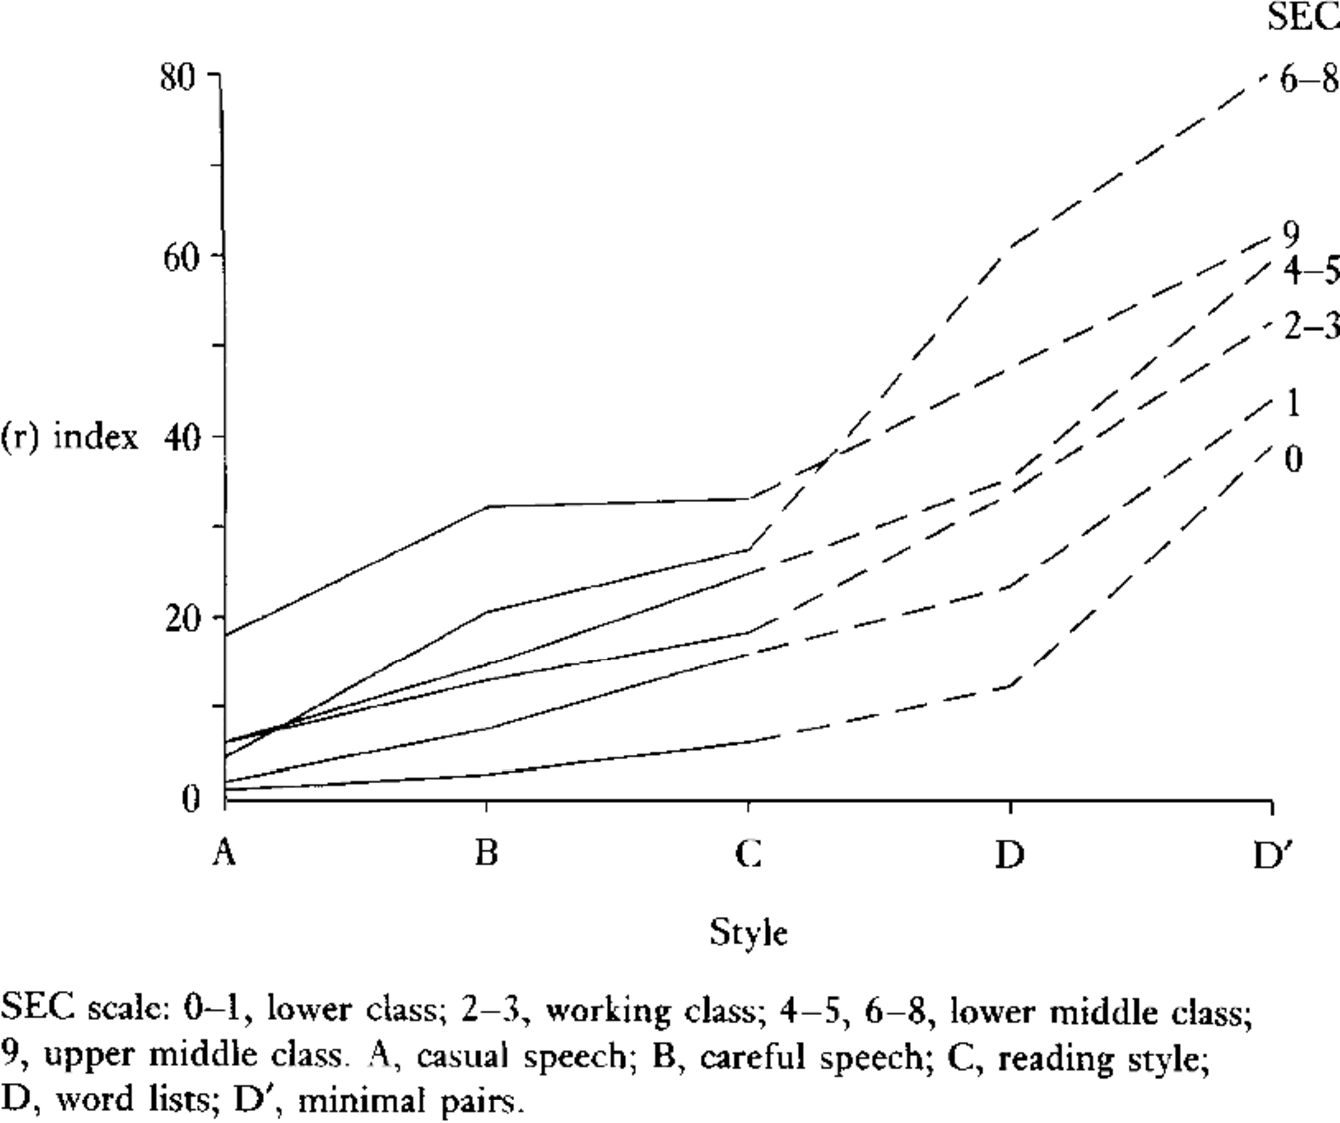
\includegraphics{LabovGraph.pdf}
\end{figure}
\end{verbatim}

\item <2-> Graphic width can be controlled with \texttt{[width=...]} option.
\begin{itemize}
\item It can be an absolute value (4in) or a relative value (.95\textbackslash textwidth)
\end{itemize}
\end{itemize}
\end{frame}

%Graphics 2
\begin{frame}[fragile]
\frametitle{Graphics options}

\begin{itemize}
\item <1-> Some more graphics options:

\begin{verbatim}
\usepackage{graphicx}
...
\begin{figure}[H]
    \centering
    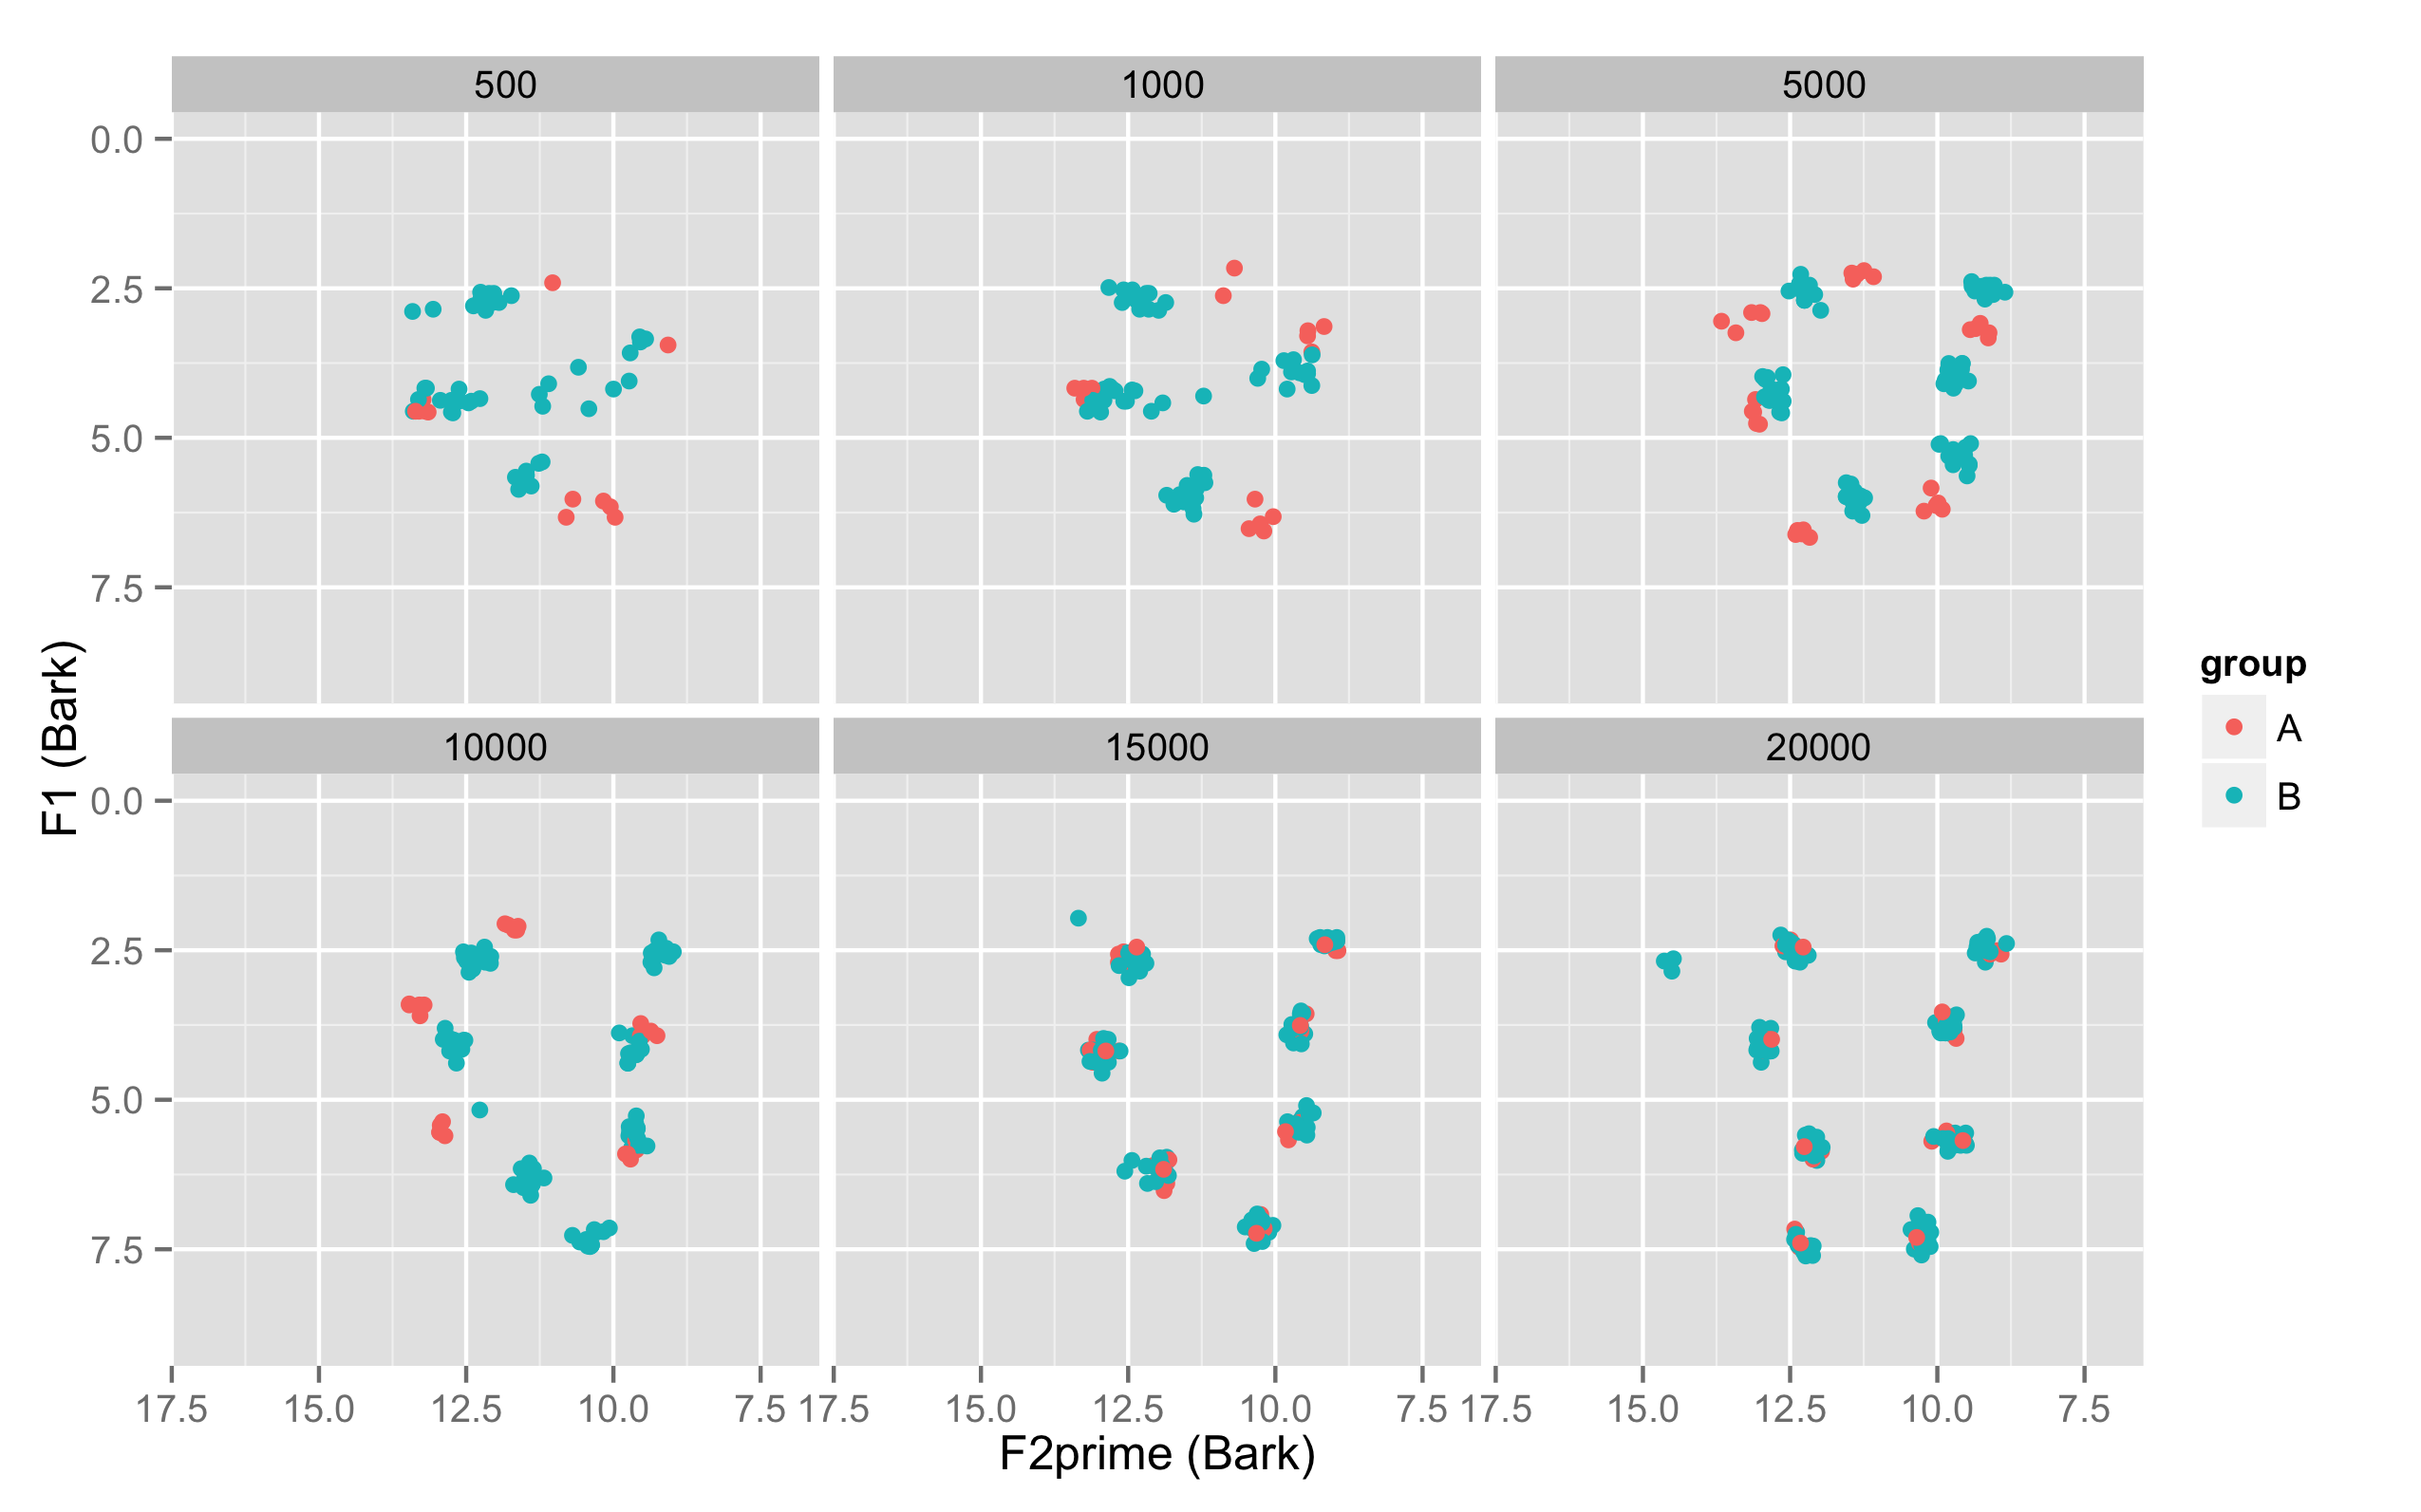
\includegraphics[width=...]{VowelSpace.png}
    \caption{...}
    \label{...}
\end{figure}
\end{verbatim}

\item <2-> \texttt{H} requires the package \texttt{float} and inserts a graphic in that exact spot---\texttt{h} will only attempt to put a graphic in that spot. \texttt{!htbp} allows a figure to be placed here \emph{h}, at the top \emph{t}, at the bottom \emph{b}, or on a float page \emph{p}.
\end{itemize}
\end{frame}

\subsection{References}
%Cross-references
\begin{frame}[fragile]
\frametitle{Cross references}

\begin{itemize}
\item <1-> \texttt{\textbackslash label\{...\}} is used to label objects for cross-reference.
\item <2-> These objects can then be referred to with the \texttt{\textbackslash ref\{...\}} command.
\item <3-> You can label graphics, tables, sections, pages, etc. 
\end{itemize}
\end{frame}

\subsection{Tables}
%Tables
\begin{frame}[fragile]
\frametitle{Tables}

\begin{itemize}
\item <1-> Tables are enclosed in the \texttt{tabular} environment.
\begin{verbatim}
\begin{tabular}{c|c|c}
    1 & 2 & 3\\
\end{tabular}
\end{verbatim}
\item <2-> \texttt{\&} separates cells and \texttt{\textbackslash\textbackslash} ends the row.
\item <3-> \texttt{\{c|l|r\}} controls the alignment of the text in each column.
\item <4-> Horizontal dividers are marked with \texttt{|} and horizontal dividers can be created with \texttt{line} between rows. 
\end{itemize}
\end{frame}

%Tables 2
\begin{frame}[fragile]
\frametitle{Tables}

\begin{itemize}
\item <1-> Tables can be embedded in the \texttt{table} environment.
\begin{verbatim}
\begin{table}
    \caption{...}
    \label{table:...}
    \begin{tabular}{c|c|c}
    ...
    \end{tabular}
\end{table}
\end{verbatim}
\item <2-> This allows you to add captions/titles and references.
\end{itemize}
\end{frame}

\subsection{Citations}

\begin{frame}[fragile]
\frametitle{natbib}   
\begin{itemize}
	\item <1-> \texttt{natbib} is a package for creating bibliographies and in-text citations.
	\item <2-> It (and the built-in) citation system use a .bib file, which stores your bibliography
	\item <3-> Programs like Mendeley can manage your .bib file automatically
	\item <4-> You can specify which citation style you'd like using \texttt{\textbackslash bibliographystyle\{\ldots\}} and by specifying \texttt{unified} for linguistics, \texttt{apalike} for APA, \texttt{chicago} for Chicago style, etc.
\end{itemize}
\end{frame}

\begin{frame}[fragile]
\frametitle{natbib}   
\begin{itemize}
	\item <1-> There are many ways to cite things:
	\item <1-> \begin{itemize}
			\item \texttt{\textbackslash citep\{\ldots\}} for (Author, Year)
			\item \texttt{\textbackslash citet\{\ldots\}} for Author (Year)
			\item \texttt{\textbackslash citep\{paper1,paper2\}} for (Author1, Year; Author2, Year)
		\end{itemize}
	\item <2-> Cheat sheet for citation commands: \url{http://merkel.zoneo.net/Latex/natbib.php}
	\item <3-> Unified style sheet for linguistics: \url{https://linguistlist.org/pubs/tocs/JournalUnifiedStyleSheet2007.pdf}
\end{itemize}

\end{frame}

\section{Linguistics}

\subsection{tipa}

\begin{frame}[fragile]
\frametitle{\texttt{tipa} package}
\begin{itemize}
\item <1-> It's pretty straightforward: IPA in LaTeX
\item <2-> It looks like this:
\begin{verbatim}
\textipa{[D@ "k\super h\ae p\textcorner t\s{n}
\~\ae nd\textcorner D@ "\t{dZ}\~En\*r@
l wIl "p\r*{\*r}Ablij: goU:]}
\end{verbatim}
\item <3-> Which produces: \textipa{[D@ "k\super h\ae p\textcorner t\s{n} \~\ae nd\textcorner D@ "\t{dZ}\~En\*r@\textsuperimposetilde{l} wI\textsuperimposetilde{l} "p\r*{\*r}Ablij: goU:]}
\end{itemize}
\end{frame}

\begin{frame}[fragile]
\frametitle{\texttt{tipa} practice}
\begin{itemize}
\item Try typesetting: \textipa{[haU du aI meIk aI pi eI sImb@lz In leItEk]}
\item Or: \textipa{[maI: "HUzb@\=*nSUd\textcorner \ae \r*v bOt\textcorner p\super h@t\super heI:RoU\r*z]}
\end{itemize}
\end{frame}

%Covington
\subsection{gb4e}

\begin{frame}[fragile]
\frametitle{\texttt{gb4e} package}
\begin{itemize}
\item <1-> gb4e introduces the \texttt{exe} environment.
\item This allows you to embed nearly anything in an environment with a typical linguistics citation number: (x)
\item It looks like:
\begin{verbatim}
\begin{exe}
    \ex
    \begin{table}
    ...
    \end{table}
    \label{...}
\end{exe}
\end{verbatim}
\end{itemize}
\end{frame}

\begin{frame}[fragile]
\frametitle{\texttt{gb4e} package}
\begin{itemize}
\item <1-> Glosses are introduced using the \texttt{\textbackslash gll} command.
\item It looks like:
\begin{verbatim}
\begin{exe}
    \ex{\gll Mi griast der Bua, (der) wo aus Minga kummt.\\
    me.\textsc{acc} greets the.\textsc{m.nom} boy who.\textsc{m.nom} that from Munich comes\\
    \glt `The boy who comes from Munich greets me.'}
\end{exe}
\end{verbatim}
\end{itemize}
\end{frame}

\begin{frame}[fragile]
\frametitle{\texttt{gb4e} package}
\begin{itemize}
\item <1-> This code produces:
\begin{figure}[H]
    \centering
    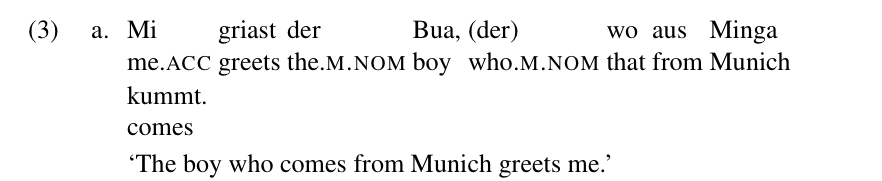
\includegraphics[width=.75\textwidth]{gb4e.png}
\end{figure}
\item <2-> Use curly brackets to group multiple words, or empty curly brackets to skip words.
\end{itemize}
\end{frame}

\begin{frame}[fragile]
\frametitle{\texttt{gb4e} package}
\begin{itemize}
\item <1-> Lists can be embedded within the example environment using the \texttt{xlist} environment:
\begin{verbatim}
\begin{exe}
    \ex
    \begin{xlist}
    \ex{...}
    \ex{...}
    \ex{...}
    \end{xlist}
\end{exe}
\end{verbatim}
\end{itemize}
\end{frame}

\begin{frame}[fragile]
\frametitle{\texttt{gb4e} package}
\begin{itemize}
\item <1-> Examples can be labeled and cross-referenced using the \texttt{\textbackslash label\{...\}} and \texttt{\textbackslash ref\{...\}} commands.
\item <2-> The \texttt{\textbackslash label\{...\}} command must come \emph{after} the example:
	\begin{verbatim}
	   \ex{Mi griast der Bua, (der) wo
	   aus Minga kummt.}\label{ex:MascNom}
	\end{verbatim}
\item <3->	Check out the \texttt{\textbackslash exr}, \texttt{\textbackslash exp}, and \texttt{\textbackslash exi} commands for other useful ways of labeling and referencing examples.
\end{itemize}
\end{frame}

\subsection{qtree}

\begin{frame}[fragile]
\frametitle{\texttt{qtree} package}
\begin{itemize}
\item <1-> qtree lets you make...trees!
\item <2-> The code looks like this:
\begin{verbatim}
\Tree [.DP [.D des ] [.$n$P
\qroof{Oachkatzl}.$n$P [.CP
\qroof{des}.DP [.C [.C wo ] 
[.TP \qroof{$\langle des
\rangle$}.DP [.T \qroof{$\langle
des \rangle$ I gfangn hab}.$v$P T ] ] ] ] ] ]
\end{verbatim}
\item <3-> It's fairly straightforward once you get the hang of it.
\begin{itemize}
	\item[$\rightarrow$] It's basically standard syntactic bracketing
\end{itemize}
\end{itemize}
\end{frame}

\begin{frame}[fragile]
\frametitle{\texttt{qtree} package}
\begin{itemize}
\item <1-> The code on the last slide produces:
\begin{figure}[H]
    \centering
    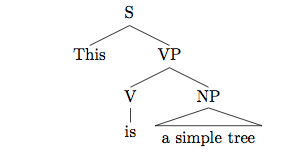
\includegraphics[width=.75\textwidth]{QTree.png}
\end{figure}
\item <2-> Try bracketing something yourself
\end{itemize}
\end{frame}

\subsection{knitr}

\begin{frame}[fragile]
\frametitle{knitr}
	\begin{itemize}
		\item <1-> \texttt{http://yihui.name/knitr/}
		\item <1-> knitr (an extension of Sweave) is a way to incorporate R code into your documents.
		\item <2-> This allows you to include dynamically-generated tables, figures, and references.
		\item <3-> The goal is transparent and reproducible research.
	\end{itemize}
\end{frame}

\begin{frame}[fragile]
\frametitle{knitr}
\begin{itemize}
	\item <1-> knitr documents can be written directly in RStudio, or in something like Sublime Text with the \texttt{SublimeKnitr} plugin.
	\item <2-> Example:

\end{itemize}
\end{frame}

\section{Resources}
\begin{frame}[fragile]
\frametitle{\LaTeX\ resources}

\begin{itemize}
\item \url{http://en.wikibooks.org/wiki/LaTeX/}
\item Twitter: @TeXtip
\item LaTeX4Ling: \url{http://www.essex.ac.uk/linguistics/external/clmt/latex4ling/}
\item Google (of course)
\end{itemize}

\end{frame}

\end{document}
